\chapter{Users Perspective}
\label{users_perspective}
	\section{Introduction}
		In this section, we will start our exploration of the application and its features. As the nature of the requirements of this
		the system is complicated. Unavoidably the system will be complex as well. Taking this into consideration, we will follow a natural top-to-bottom
		approach explaining its internals, starting as end-users and seeing the system as a black box. In this section, we will analyze its 
		functionality from the user's perspective. This section may also serve as an instruction manual for the end-user as it contains everything needed
		for an inexperienced user to start working with the software.
	\section{Login and Authentication}
		\begin{figure}[H]
			\iftrue
			\centering
			\caption{Login Screen}
			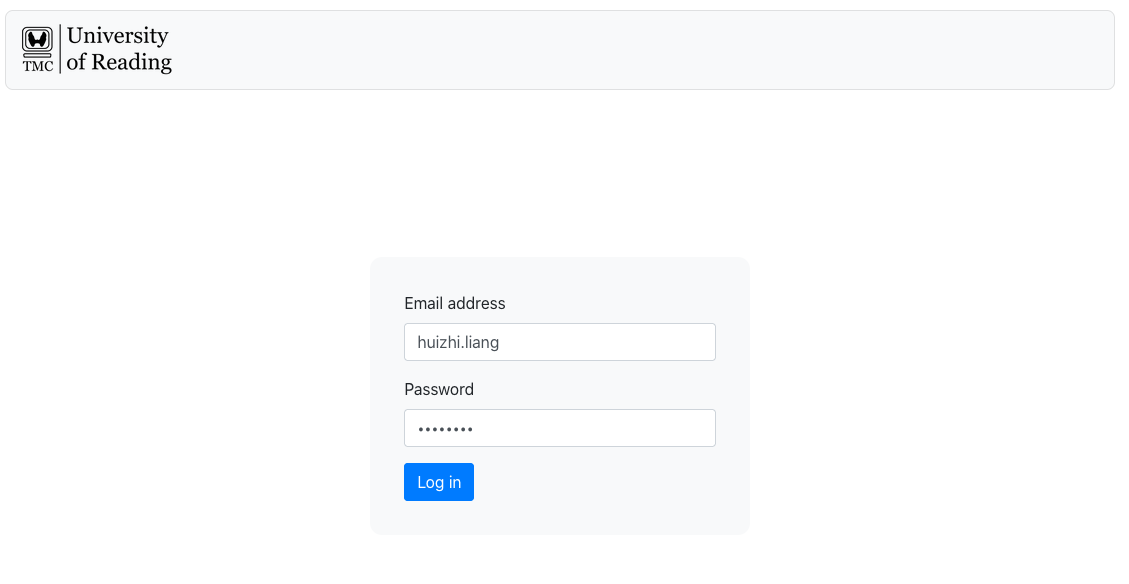
\includegraphics[scale=0.3]{figures/login}
			\fi
		\end{figure}
		The login screen is the first screen that our end-users will encounter. Here a username and a password is required to be given by the 
		user to log in. The Credentials of the user remain encrypted during the process of login, as the system utilizes an HTTPS[\cite{rfc2818}] 
		protocol for its connection, this is essential for the first non-functional requirement about security (see \ref{non-functional-requirements}).
		The username and the password may be requested by the system administrator or the NOC\footnote{Network Operations Center} of the hospital.
	\section{Home}
		\begin{figure}[H]
			\iftrue
			\centering
			\caption{Home Screen}
			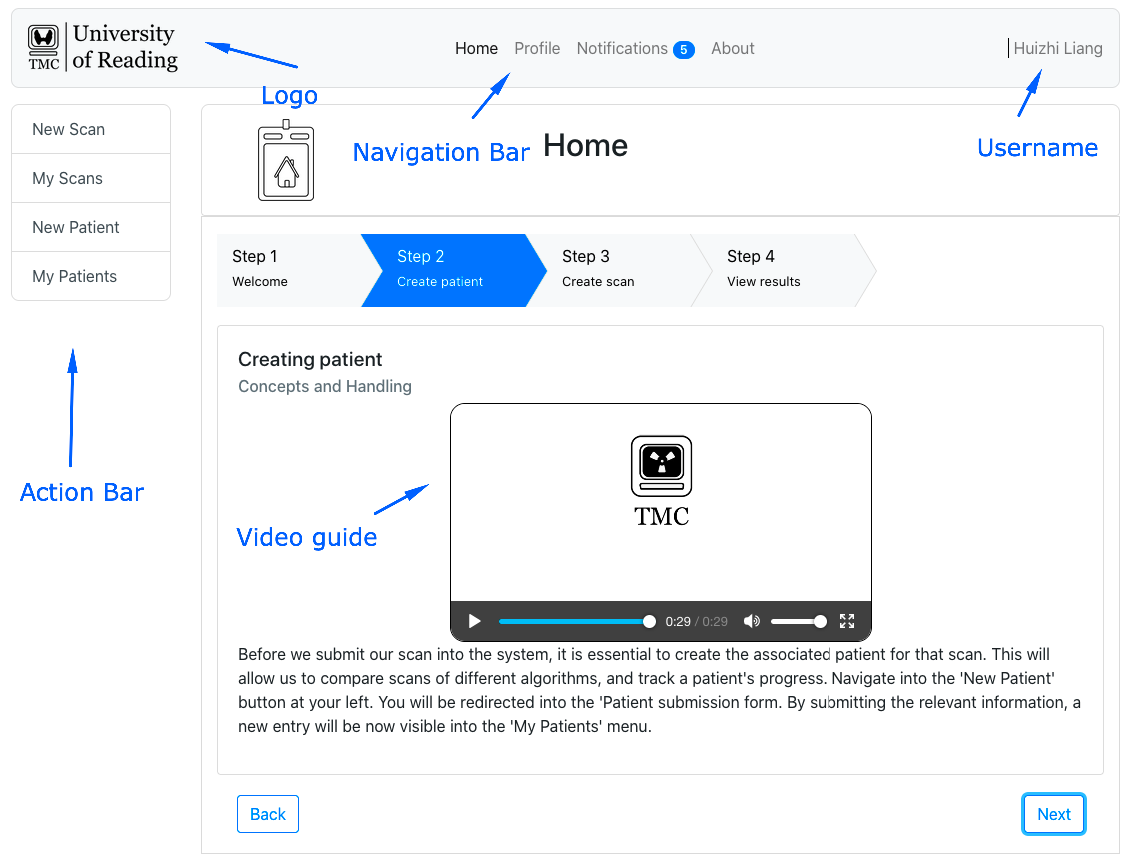
\includegraphics[scale=0.3]{figures/home}
			\fi
		\end{figure}
		After the login process is completed. The user encounters the 'home screen. From here, it is possible to navigate to the features of the software
		as well as learn about how the software can be utilized through detailed guides and videos. The UI/UX\footnote{User Interface-User Expieriance} 
		has been designed to be as user-friendly as possible. Some areas of interest are given below.
		\begin{center}
			\begin{tabular}{ |c|c| } 
				\hline
				Action bar & The Actions that can be performed using the software can be accesed from here.\\
				Navigation bar & General information and notification bar. \\
				\hline
			\end{tabular}
		\end{center}
	\section{Navigation bar}
		In this section, we will briefly look at the options under the Navigation bar.
		\subsection{Profile}
			\label{profile-screen}
			\begin{figure}[H]
				\iftrue
				\centering
				\caption{Profile}
				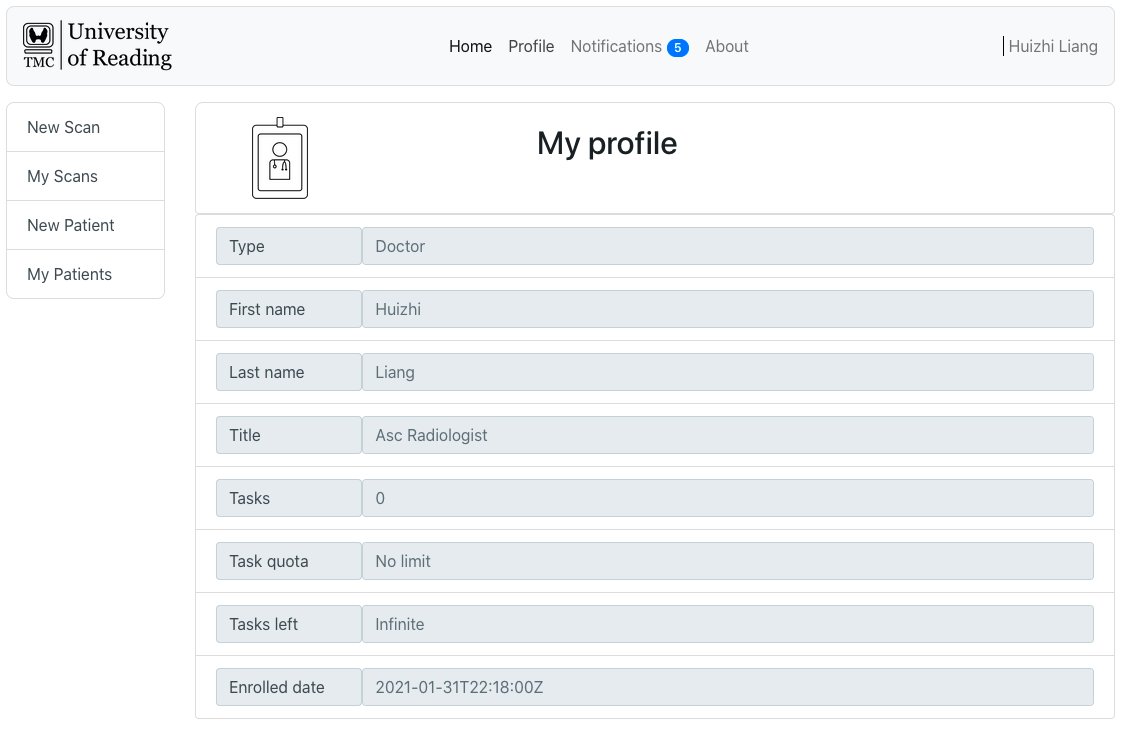
\includegraphics[scale=0.3]{figures/profile}
				\fi
			\end{figure}
			In the profile section, the user can see its associated information, saved on the registration date. 
			The information for security reasons cannot be altered by the user itself, but only after a request to 
			the system administrator or NOC\footnote{Network Operations Center}.
		\subsection{Notifications}
			\label{notification-screen}
			\begin{figure}[H]
				\iftrue
				\centering
				\caption{Notifications}
				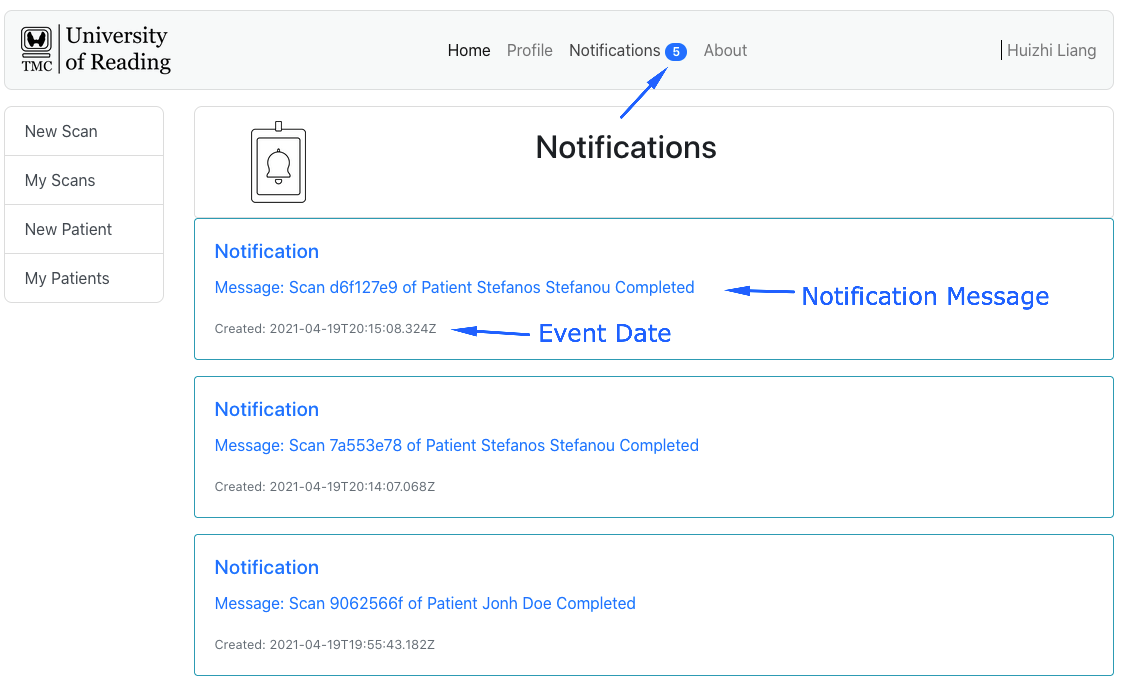
\includegraphics[scale=0.3]{figures/notifications}
				\fi
			\end{figure}
			In the notification section, helpful information about events that may interest the end-user can be found, 
			such as the fact that uploaded scan results are ready to view. 
		\subsection{About}
			\begin{figure}[H]
				\iftrue
				\centering
				\caption{About}
				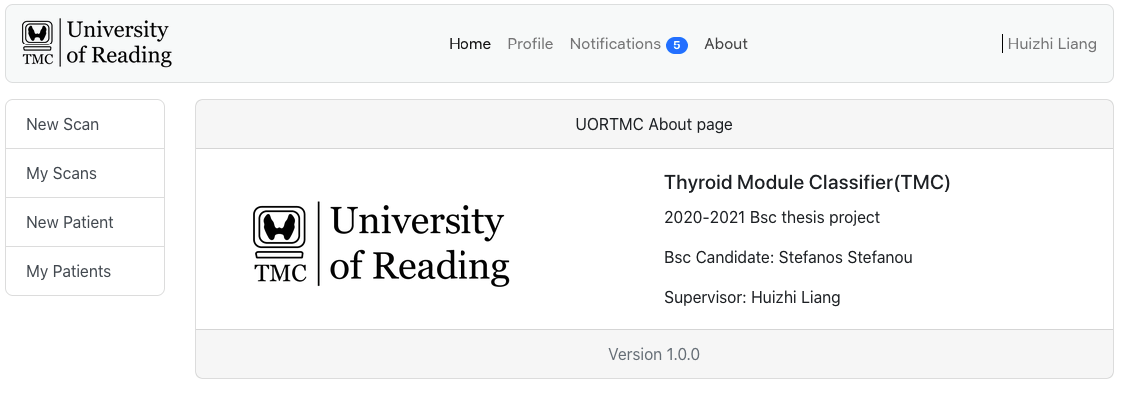
\includegraphics[scale=0.3]{figures/about}
				\fi
			\end{figure}
			From here, a user may found helpful information about the software, such as the current version.
	\section{Action Bar}
		In this section, we will briefly look at the options under the Action Bar.
		\subsection{My Patients}
			\label{my-patients}
			\begin{figure}[H]
				\iftrue
				\centering
				\caption{Patients List}
				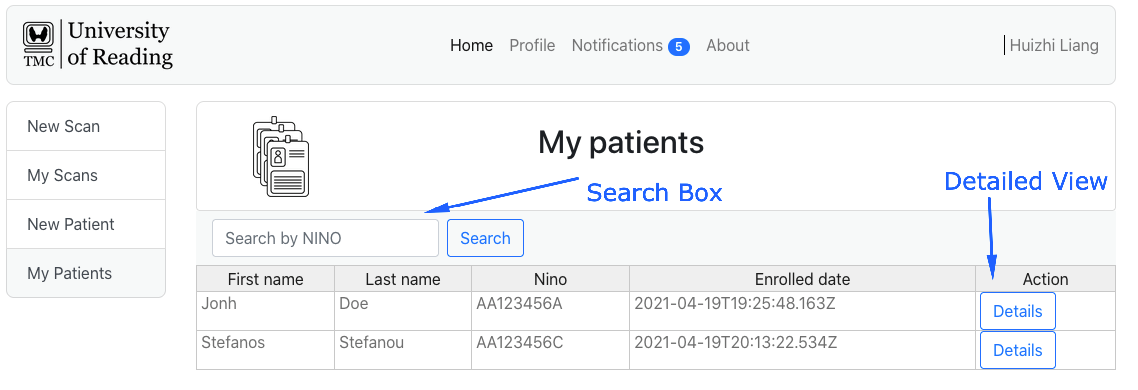
\includegraphics[scale=0.3]{figures/mypatients}
				\fi
			\end{figure}
			This page will show us a list of the currently registered patients. Each end-user(doctor) may only see its 
			patients and not others. The end-user can search the list based on NiNo[\cite{nino-format}] of the given 
			patient for convenience. The end-user can also view the details of a given patient and record various 
			notes/comments for that patient by clicking the 'Details' button on his selected patient, as seen below. 
			Finally, clicking the button 'View Scans' can see the specific patient history of uploaded scans.
			\begin{figure}[H]
				\iftrue
				\centering
				\caption{Patient Details}
				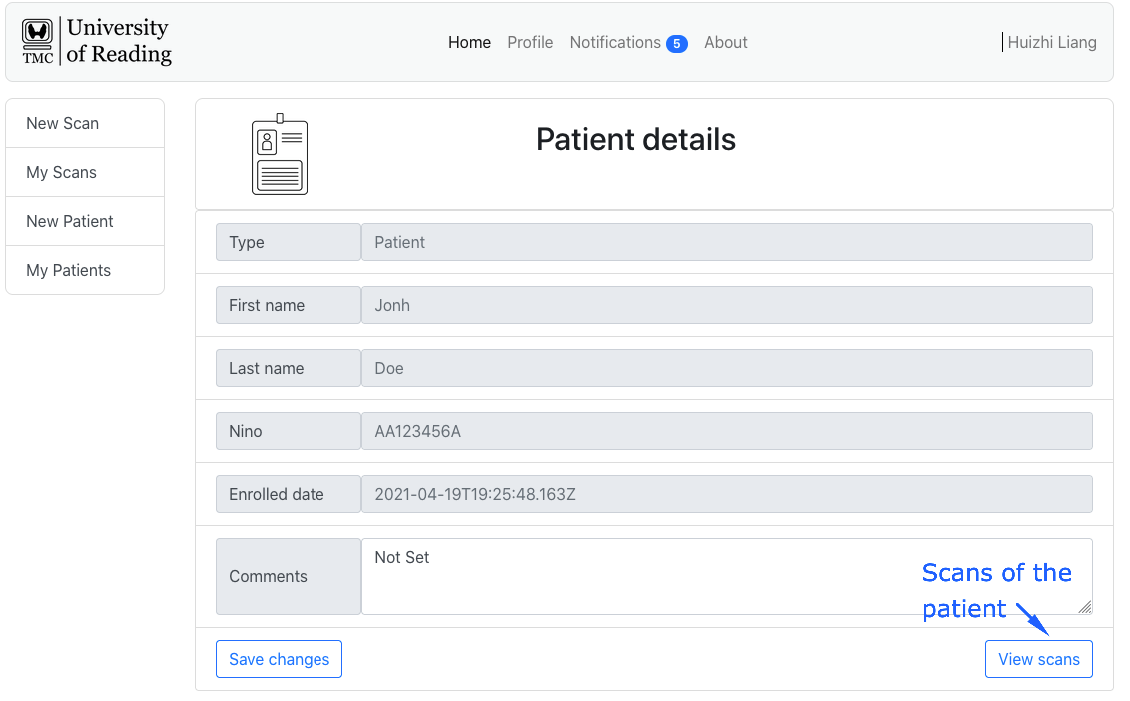
\includegraphics[scale=0.3]{figures/mypatients2}
				\fi
			\end{figure}
		\subsection{New Patient}
			\label{patient-submission}
			\begin{figure}[H]
				\iftrue
				\centering
				\caption{New Patient}
				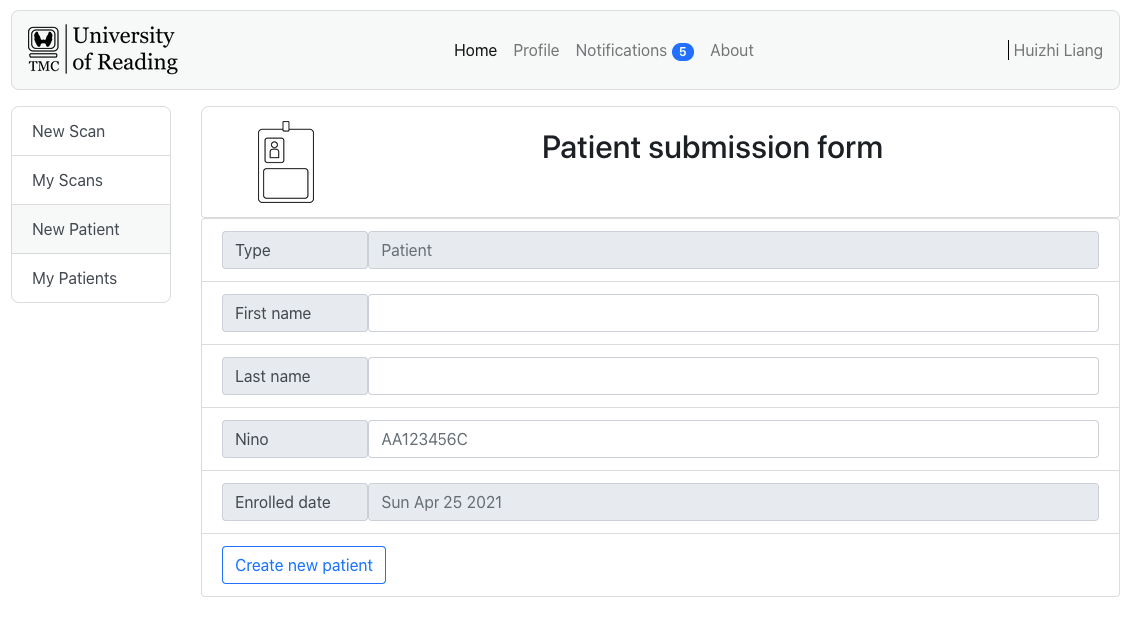
\includegraphics[scale=0.3]{figures/newpatient}
				\fi
			\end{figure}
			By clicking the 'New Patient' action on Action Bar, the user can register a new patient on the system. The following conditions need to 
			be met for the operation to be successful.
			\begin{itemize}
				\item First name length should be more than 2 characters, encoded as UTF-8[\cite{rfc3629}]
				\item Last name length should be more than 2 characters, encoded as UTF-8[\cite{rfc3629}]
				\item NiNo should be at standard format [\cite{nino-format}], encoded as UTF-8[\cite{rfc3629}]
			\end{itemize}
			Failing to fulfill these constraints should lead to an error, as shown below.
			\begin{figure}[H]
				\iftrue
				\centering
					\caption{New Patient Error}
				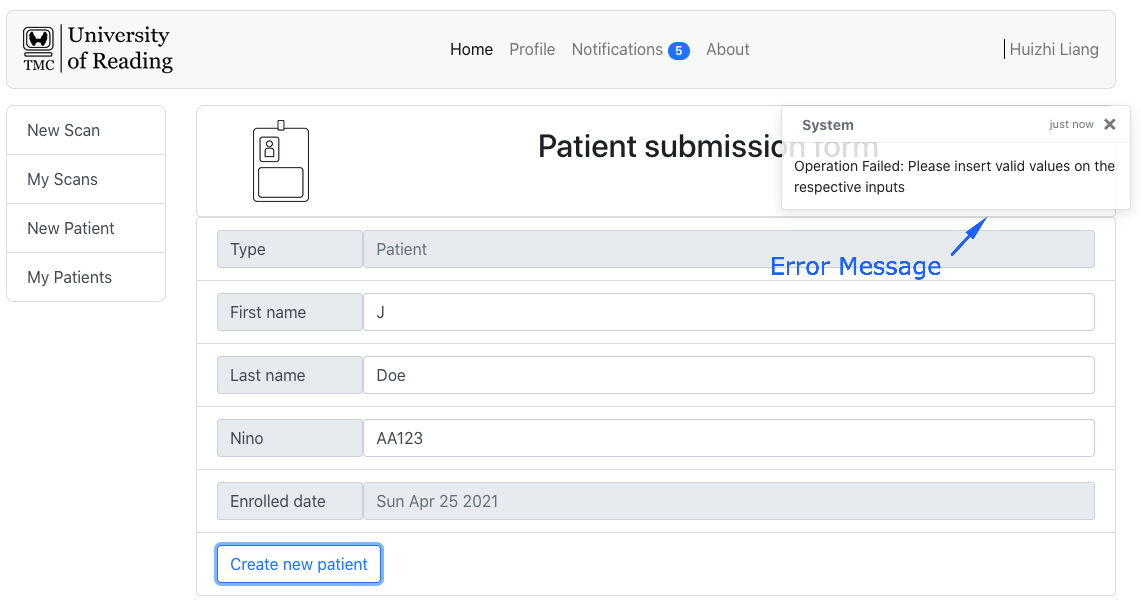
\includegraphics[scale=0.3]{figures/newpatient-error}
				\fi
			\end{figure}
		\subsection{My Scans}
			\label{my-scans}
			\begin{figure}[H]
				\iftrue
				\centering
				\caption{My Scans}
				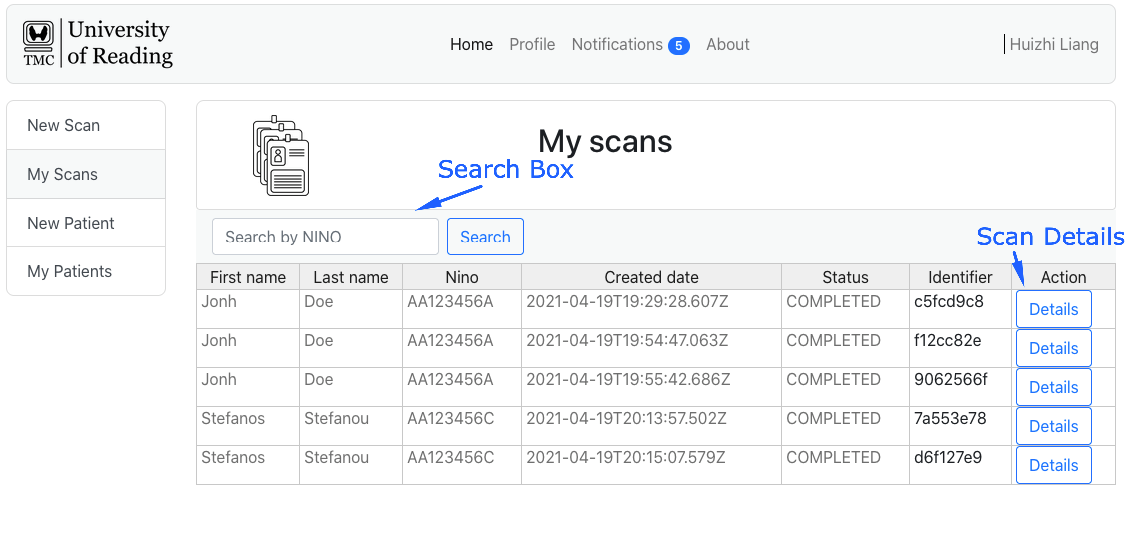
\includegraphics[scale=0.3]{figures/myscans}
				\fi
			\end{figure}
			'MyScans' are a complete list with all submitted scans for a given end-user. 
			The user can search for the scans of a specific patient by using the search box and viewing the 
			scan results (if a given scan is complete) by clicking the 'Details' button of the scan in question.
			\begin{figure}[H]
				\iftrue
				\centering
				\caption{Scan results}
				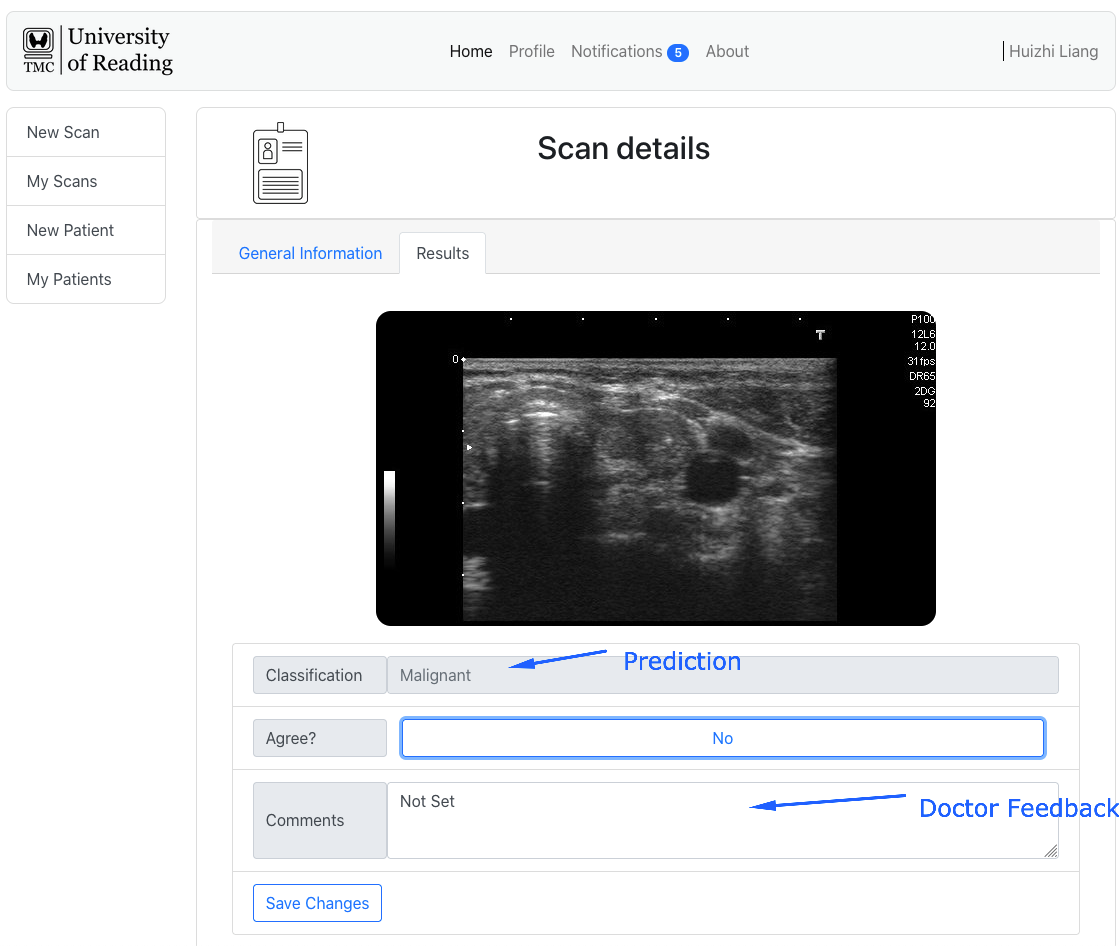
\includegraphics[scale=0.3]{figures/myscans-details}
				\fi
			\end{figure}
		\subsection{New Scan}
			\label{new-scan}
			\begin{figure}[H]
				\iftrue
				\centering
				\caption{New Scan}
				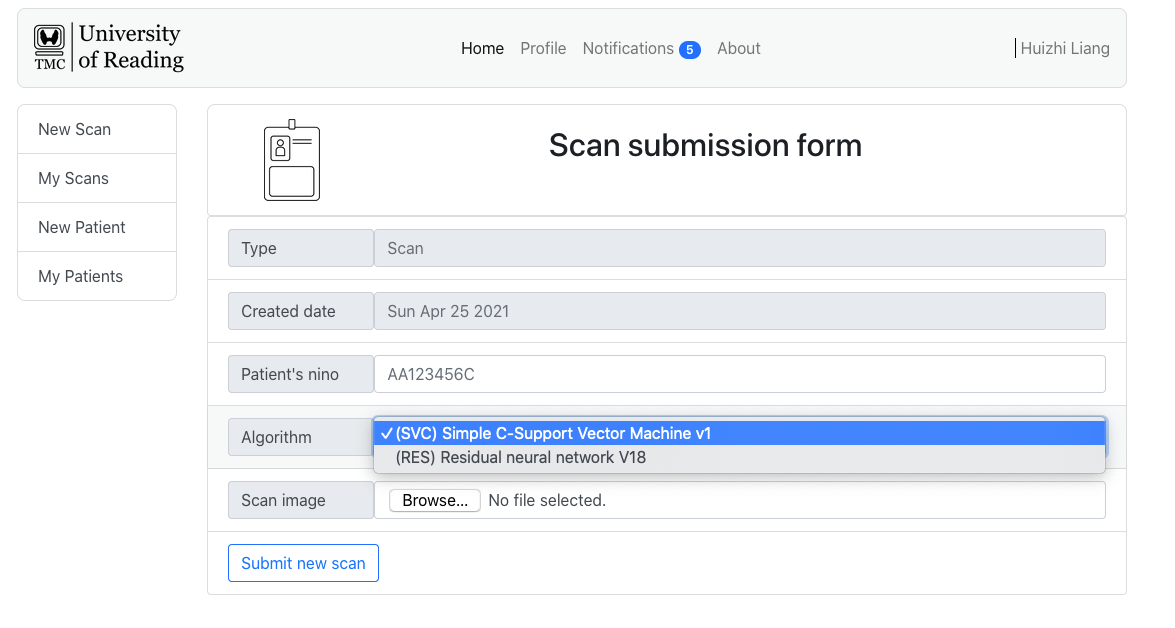
\includegraphics[scale=0.3]{figures/newscan}
				\fi
			\end{figure}
			By clicking the 'New Scan' action, the user is redirected into the scan submission form. Here it is possible to 
			submit a new ultrasound image for a given patient.The user can also select the algorithm for performing the 
			classification (see \ref{prediction-service}). The operation to be completed should meet the following criteria.
			\begin{itemize}
				\item Patients Nino should be in standard format[\cite{nino-format}] and encoded as UTF-8[\cite{rfc3629}]
				\item Scan Image should be a ISO/IEC 10918-1/JPEG[\cite{jpeg-iso10918-1}] format with 360x560 resolution. The image name
				should be encoded as UTF-8[\cite{rfc3629}]
			\end{itemize}
			Failing to fulfill these constraints should lead to an error, as shown below.
			\begin{figure}[H]
				\iftrue
				\centering
				\caption{Invalig image format (PNG) error}
				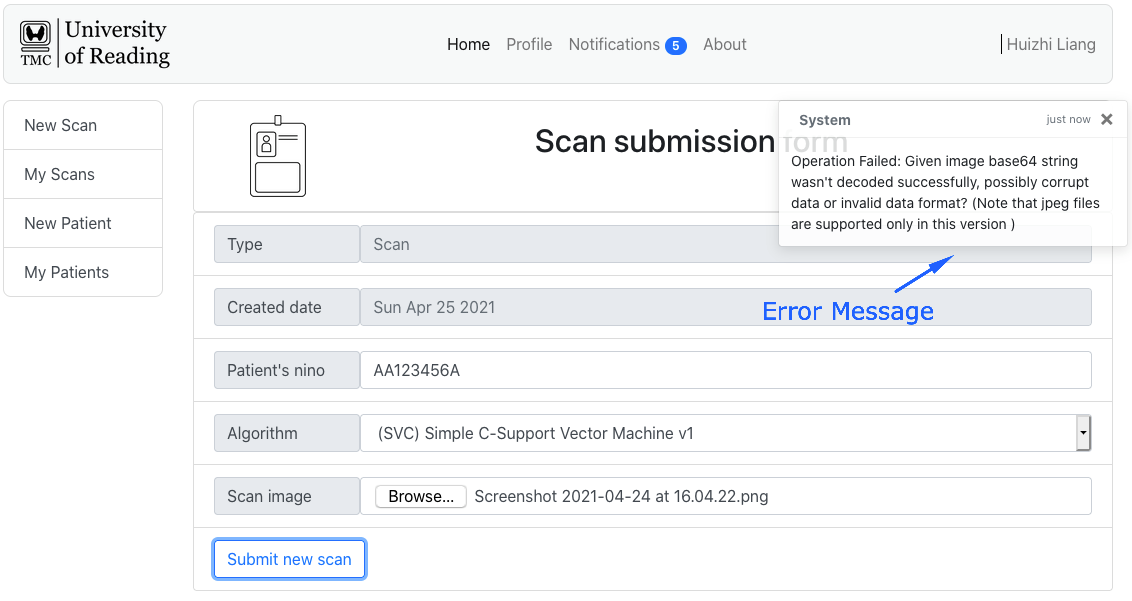
\includegraphics[scale=0.3]{figures/newscan-error}
				\fi
			\end{figure}
			
			
			
			
			
			
			
		
	



